% !TeX root = incremental_SS_Translation.tex
\chapter{Kalpasthāna: Introduction}

\section{The Sequence of Chapters}
\label{kalpa-chapter-sequence}
The Nepalese version of the \SS\ reverses the sequence of chapters 6 and 7.  

\begin{table}[h]
    \centering
     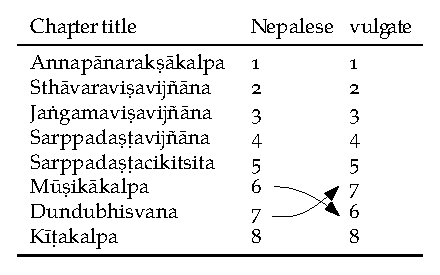
\includegraphics[width=0.65\linewidth]{chapters/media/kalpa}
%    \begin{tabular}{lll}
%    \emph{Chapter title} & \emph{Nepalese} & \emph{vulgate}   \\
%    \toprule
%      Annapānarakṣākalpa   &  1 &  1 \\
%     Sthāvaraviṣavijñāna & 2 &  2\\
%     Jaṅgamaviṣavijñāna &  3 & 3 \\
%     Sarppadaṣṭavijñāna & 4  &  4 \\
%     Sarppadaṣṭacikitsita & 5 & 5 \\
%     Mūṣikākalpa &  {6} & \textbf{7} \\
%     Dundubhisvana & {7} & \textbf{6} \\
%     Kīṭakalpa & 8 & 8 \\
%    \bottomrule  
%    \end{tabular}
\end{table}

% TODO: \usepackage{graphicx} required
%\begin{figure}
%    \centering
%    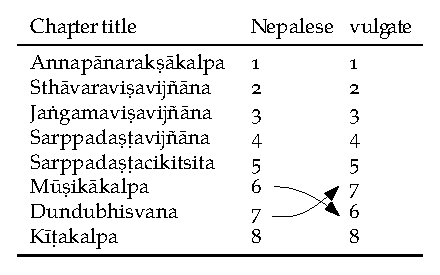
\includegraphics[width=0.65\linewidth]{chapters/media/kalpa}
%    \caption{}
%    \label{fig:kalpa}
%\end{figure}

\noindent
This difference in sequence does not have an immediately obvious 
significance.